\documentclass{article}
\usepackage[spanish]{babel}
\usepackage[utf8]{inputenc}
\usepackage{graphicx}
\usepackage{fancyhdr}
\usepackage{amssymb,amsmath,amsthm}
\usepackage{geometry}
\usepackage{enumerate}
\usepackage{float}

%Comandos:
\newcommand{\R}{\mathbb{R}}
\newcommand{\N}{\mathbb{N}}

% Configuración de página:
\geometry{letterpaper,margin=2cm,tmargin=3cm}

\fancypagestyle{plain}{
	\fancyhead[L]{Universidad de Chile\\Facultad de Ciencias Físicas y Matemáticas\\MDS7203 Modelos Generativos Profundos}
	\fancyhead[R]{
\includegraphics[height=1.5cm]{images/fcfm}}
}
\pagestyle{fancy}{
\fancyhead[L]{Facultad de Ciencias Físicas y Matemáticas}
\fancyhead[R]{Universidad de Chile}
}

%Título:
\title{\bfseries{Control de Lectura nº3}\vspace{0.5cm}}
\author{\textbf{Nombre:} \rule{12cm}{0.4pt}}

% Documento:
\begin{document}
\maketitle

\hspace{-0.5cm}\textbf{Instrucciones:} Responda las siguientes preguntas de forma breve y precisa. El control de lectura tiene una duración de 20 minutos y no está permitido el uso de apuntes ni dispositivos electrónicos.

\section*{Agentes basados en LLMs}
\begin{enumerate}[{\bf P1.}]
	\item Considere un LLM post-entrenado para uso agéntico. Explique brevemente el bucle de inferencia que se debe implementar para ejecutar las acciones \textit{solicitadas} por el LLM.
\end{enumerate}

\section*{Redes generativas adversarias}
\begin{enumerate}[{\bf P1.}]
	\item Explique con sus palabras cómo funciona una GAN. Su respuesta debe mencionar el rol del generador y del discriminador, y cómo interactúan durante el entrenamiento.
	\item En el entrenamiento del generador $G_\theta:\R^L\to\R^D$ de una GAN, la función de pérdida original basada en la verosimilitud del discriminador es la siguiente:
	\begin{equation*}
		\min_\theta\;\mathbb{E}_{z\sim\mathcal{N}(0,\mathrm{I}_L)}\!\left[\underbrace{\log\!\left(1-D_\phi(G_\theta(z))\right)}_{\text{prob. clasificar como falsa}}\right] + \text{constante}.
	\end{equation*}
	Esta versión se dice \textit{saturante} y, en la práctica, es cambiada por una versión \textit{no saturante}:
	\begin{equation*}
		\max_\theta\;\mathbb{E}_{z\sim\mathcal{N}(0,\mathrm{I}_L)}\!\left[\underbrace{\log D_\phi(G_\theta(z))}_{\text{prob. clasificar como verdadera}}\right] + \text{constante}.
	\end{equation*}
	La siguiente figura muestra la diferencia entre ambas versiones, donde en el eje de las abscisas se representa la probabilidad entregada por el discriminador, $d = D_\phi(G_\theta(z))\in[0,1]$:
	\begin{figure}[H]
		\centering
		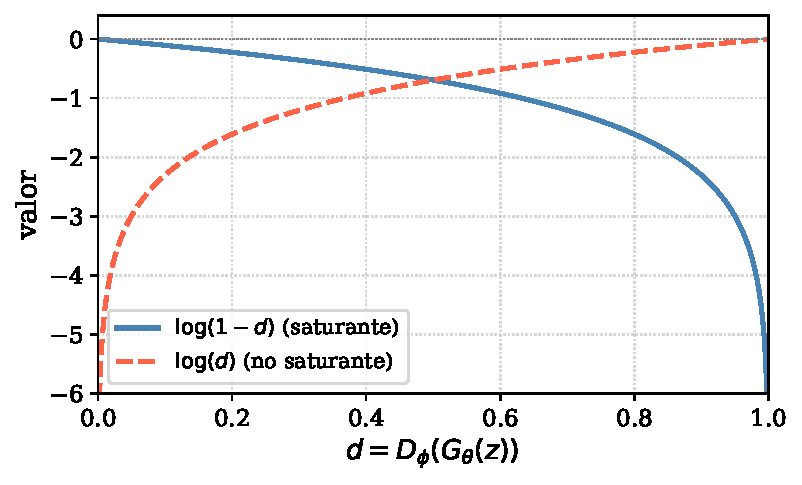
\includegraphics[width=0.4\textwidth]{images/log_saturation}
	\end{figure}
	Ayudándose del gráfico, explique por qué en la práctica se prefiere utilizar la versión no saturante. Considere cómo se comportan los gradientes de cada función de pérdida en el comienzo del entrenamiento.
\end{enumerate}

\end{document}
